\thispagestyle{fancy}
\chapter{Kravspecifikation}
I denne del af bachelor-forbedrelsesjournalen vil projektets foreløbige funktionelle krav blive gennemgået. Kravene, der her bliver gennemgået, skal ses som midlertidige udkast, da projektets mål ikke er endeligt fastlagt.
\\ \\
I projektets kontekstdiagram vil systemets overordnede struktur blive beskrevet. \\
Foreløbig er intentionen at projektet opdeles i tre særskilte dele:\\
\begin{enumerate}
	\item En dataopsamlingsdel, hvor data kan opsamles, organiseres og glemmes, så det kan anvendes af de øvrige dele af projektet
	\item En machine-lerning-del, hvor den indsamlede data processeres. Videre skal der i denne del være mulighed for at begrænse, hvilke dele af den indsamlede data, der processeres
	\item En form for SDK-del, der kan anvendes i software, hvor der er behov for håndbevægelsesgenkendelse
	
\end{enumerate}

\section{Kontekstdiagram}
\begin{figure}[h!]
	\centering
	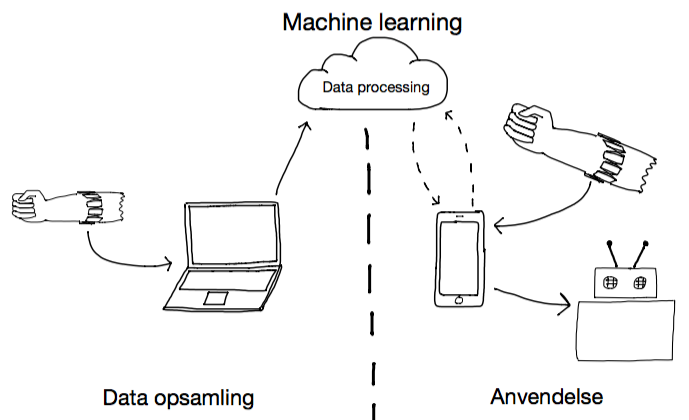
\includegraphics[width=1\textwidth]{kontekstdiagram}
	\caption{Kontekstdiagram }
	\label{fighrj}
\end{figure}
To af projektets tre dele adskilles i kontekstdiagrammet af en stiplet linje, nemlig dataopsamlingsdelen og anvendelsesdelen. Derudover ses machine-learning-delen i toppen af figuren, og er forbundet til de to øvrige dele. Machine-learning-delen er  ansvarlig for at kende forskellige håndbevægelser, og kan derved melde hvilke bevægelser der er opfanget, til software der bruger den. Derudover lærer Machine-learing-delen nye bevægelser vha. dataopsamlings-delen.

\section{User case diagram}
Følgende use case diagram beskriver, projektets aktører i relation til de enkelte use cases, der foreløbigt er tiltænkt projektet.\\
\begin{figure}[h!]
	\centering
	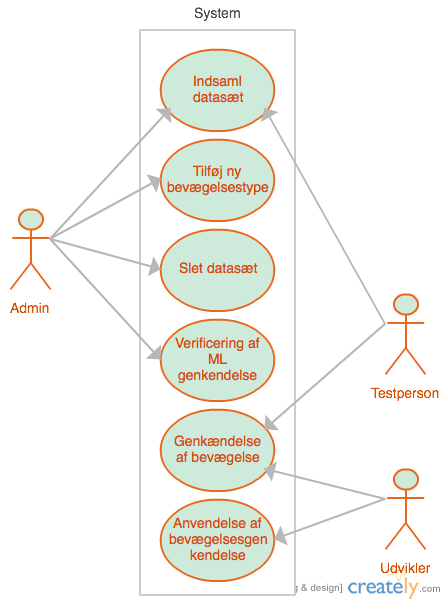
\includegraphics[width=0.75\textwidth]{UseCaseDiagram}
	\caption{Systemets Use Case Diagram}
\end{figure}

\section{Aktørbeskrivelse}
Heunder gennemgåes systemts identificerede aktører.
\subsubsection*{Admin}
I dette system er Admin en person, der optager og gemmer ny bevægelsesdata og giver machine learning algoritmen adgang til den. Videre kan Admin modificere på algoritmen.

\subsubsection*{Testperson}
En Testperson i dette system, bærer et Myo armbånd, som er forbundet til en computer el.lign.   

\subsubsection*{Udvikler}
En udvikler ( eller softwareudvikler ) er, i dette system en softwareudvikler, som anvender håndbevægelsesgenkendelse i egen software.  

\section{Fully dressed use cases}
I dette afsnit findes detaljerede beskrivelser af projektets use cases, dog er disse ikke fuldstændig gennemarbejdet, da stadig er en vis usikkerhed om projektets endelig.
\\ \\Særlig use case 5 og 6 er illustrative og beskriver den generelle idé om at genkendelse programmet bør kunne implementeres og anvendes i tredjeparts software.
\subsection{UC 1 - Indsaml datasæt}
\begin{table}[htbp] 
	\begin{tabular}{|p{5cm}|p{9cm}|}
		\hline
		\textbf{Navn} & Indsaml datasæt \\ \hline
		\textbf{Use case ID} & U1 \\ \hline
		\textbf{initiering} & Admin initierer denne use case \\ \hline
		\textbf{Aktører} & Admin (Primær Aktør ) \\ & Testperson (Sekundær aktør) \\ \hline
		\textbf{Prækondition} & Testperson har Myo båndet på og dataindsamlings software kører \\ \hline
		\textbf{Postkondition} & Datasæt er indsamlet \\ \hline
	\end{tabular}
\end{table}
\textbf{Hovedscenarie}
\begin{enumerate}
	\item Admin trykker på knap på at starte for at starte dataindsamlingen.
	\item Testpersonen laver håndbevægelse.
	\item Admin trykker på knap for at stoppe dataindsamlingen, når håndbevægelsen er slut.
	\item Admin vælger, hvilken bevægelsestype der er blevet indsamlet og angiver hvem testpersonen er.
	\item Admin trykker på knap for at gemme datasættet.
\end{enumerate}

\subsection{UC 2 - Tilføj ny bevægelsestype}
\begin{table}[htbp] 
	\begin{tabular}{|p{5cm}|p{9cm}|}
		\hline
		\textbf{Navn} & Tilføj ny bevægelsestype \\ \hline
		\textbf{Use case ID} & U2 \\ \hline
		\textbf{initiering} & Admin initierer denne use case \\ \hline
		\textbf{Aktører} & Admin (Primær Aktør ) \\ \hline
		\textbf{Prækondition} & Dataindsamlings softwaren kører \\ \hline
		\textbf{Postkondition} & En ny bevægelsestype er tilføjet til Dataindsamlingssoftwaren \\ \hline
	\end{tabular}
\end{table}
\textbf{Hovedscenarie}
\begin{enumerate}
	\item Admin trykker på knap for at tilføje ny bevægelsestype.
	\item Admin angiver titel for den nye bevægelsestype.
	\item Admin vælger, hvilken bevægelsestype der er blevet indsamlet og angiver hvem testpersonen er.
	\item Admin trykker på knap for at gemme bevægelsestypen.
\end{enumerate}

\subsection{UC 3 - Slet datasæt}
\begin{table}[htbp] 
	\begin{tabular}{|p{5cm}|p{9cm}|}
		\hline
		\textbf{Navn} & Slet datasæt \\ \hline
		\textbf{Use case ID} & U3 \\ \hline
		\textbf{initiering} & Admin initierer denne use case \\ \hline
		\textbf{Aktører} & Admin (Primær Aktør ) \\ \hline
		\textbf{Prækondition} & Et datasæt skal eksistere \\ \hline
		\textbf{Postkondition} & Datasæt er slettet \\ \hline
	\end{tabular}
\end{table}
\textbf{Hovedscenarie}
\begin{enumerate}
	\item Admin vælger eksisterende datasæt.
	\item Admin trykker på knap for at slette valgte datasæt.
\end{enumerate}
\newpage
\subsection{UC 4 - Verificering af ML genkendelse}
\begin{table}[htbp] 
	\begin{tabular}{|p{5cm}|p{9cm}|}
		\hline
		\textbf{Navn} & Verificering af ML genkendelse \\ \hline
		\textbf{Use case ID} & U4 \\ \hline
		\textbf{initiering} & Admin initierer denne use case \\ \hline
		\textbf{Aktører} & Admin (Primær Aktør ) \\ \hline
		\textbf{Prækondition} & ML har kategoriseret bevægelse \\ \hline
		\textbf{Postkondition} & Admin har varificeret kategorisering  \\ \hline
	\end{tabular}
\end{table}
\textbf{Hovedscenarie}
\begin{enumerate}
	\item Admin tjekker ML kategoriseringer.
	\begin{enumerate}
		\item Korrekt kategorisering: admin verificerer kategorisering.
		\begin{enumerate}
			\item Verificering gemmes.
		\end{enumerate}
		\item Ukorrekt verificiering: admin ændre kategorisering.
		\begin{enumerate}
			\item Ny kategorisering gemmes som verificeret.
		\end{enumerate}
	\end{enumerate}
\end{enumerate}

\subsection{UC 5 - Anvendelse af bevægelsesgenkendelse}
\begin{table}[htbp] 
	\begin{tabular}{|p{5cm}|p{9cm}|}
		\hline
		\textbf{Navn} & Anvendelse af bevægelsesgenkendelse \\ \hline
		\textbf{Use case ID} & U5 \\ \hline
		\textbf{initiering} & Udvikleren initierer denne use case \\ \hline
		\textbf{Aktører} & Udvikleren (Primær Aktør ) \\ \hline
		\textbf{Prækondition} & Udvikleren har bevægelsesgenkendelses SDK\\ \hline
		\textbf{Postkondition} & Udvikleren har anvendt bevægelsesgenkendelsen\\ \hline
	\end{tabular}
\end{table}
\textbf{Hovedscenarie}
\begin{enumerate}
	\item Udvikleren implementerer SDK i egen software
	\item Udvikleren anvender SDK til bevægelsesgenkendelse
\end{enumerate}

\newpage
\subsection{UC 6 - Genkendelse af bevægelse}
\begin{table}[htbp] 
	\begin{tabular}{|p{5cm}|p{9cm}|}
		\hline
		\textbf{Navn} & Genkendelse af bevægelse  \\ \hline
		\textbf{Use case ID} & U6 \\ \hline
		\textbf{initiering} & Testpersonen initierer denne use case \\ \hline
		\textbf{Aktører} & Testperson (Primær Aktør )\\ & Udvikler (Sekundær aktør) \\ \hline
		\textbf{Prækondition} & Testperson har Myo bånd på, som er forbundet til Udviklerens software \\ \hline
		\textbf{Postkondition} & Håndbevægelse er blevet genkendt\\ \hline
	\end{tabular}
\end{table}
\textbf{Hovedscenarie}
\begin{enumerate}
	\item Testperson laver håndbevægelse
	\item Myo-data sendes til softwareudviklerens software på computer el.lign.
	\item Udviklerens software processer Myo-data
	\item Myo-data genkendes
	\item Testpersonens håndbevægelse genkendes
\end{enumerate}